% Перестроение поверхности в 3d.
\subsection{Методы перестроения поверхности в трехмерном случае}\label{sec:text_1_remesh_3d}

\subsubsection{Архитектура неструктурированной поверхностной расчетной сетки}

Задача перестроения поверхности в трехмерном случае рассматривается на неструктурированной поверхностной расчетной сетке с треугольными ячейками \cite{Meshcheryakov2023GeoEvo}.
Элементами расчетной сетки являются узлы ($N$), ребра ($e$) и треугольные ячейки ($f$).
Для удобства каждый элемент сетки связан со всеми своими инцидентными элементами: так связаны между собой инцидентные узлы и ребра, узлы и ячейки, ребра и ячейки (см. рис.~\ref{fig:text_1_remesh3_architecture}).
Множество инцидентных узлов рассматриваемого ребра или ячейки будем обозначать $\mathscr{N}$, множество инцидентных ребер рассматриваемого узла или ячейки будем обозначать $\mathscr{E}$, множество инцидентных ячеек рассматриваемого узла или ребра будем обозначать $\mathscr{F}$.

\begin{figure}[ht]
\centering
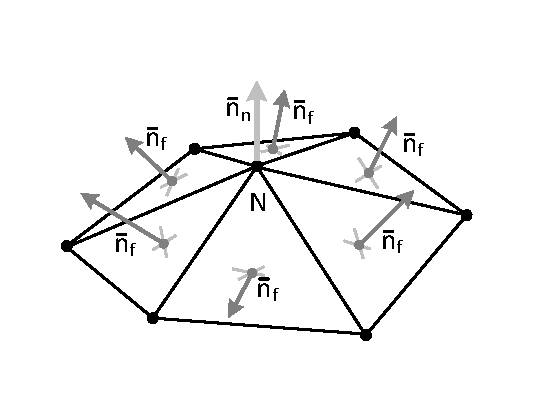
\includegraphics[width=0.5\textwidth]{pics/text_1_remesh_3d/pic_architecture.pdf}
\captionstyle{center}\caption{Архитектура расчетной сетки.}
\label{fig:text_1_remesh3_architecture}
\end{figure}

К расчетной сетке предъявляются следующие требования.
Во-первых, сетка должна быть целостной, то есть каждое ребро имеет ровно два инцидентных узла, отсутствуют изолированные и висячие узлы, а также изолированные ребра.
Во-вторых, все ячейки должны представлять собой треугольники (это гарантирует, что ячейка является плоской, так как четыре и более произвольных узлов могут не лежать в одной плоскости).
И в-третьих, рассматриваются только замкнутые сетки, представляющие собой поверхности, то есть каждое ребро имеет ровно две инцидентные ячейки (отсутствуют граничные ребра).
\begin{equation}\label{eqn:text_1_remesh3_arch}
\begin{cases}
\forall N \implies |\mathscr{E}(N)| > 2, |\mathscr{F}(N)| > 2, \\
\forall e \implies |\mathscr{N}(e)| = 2, |\mathscr{F}(e)| = 2, \\
\forall f \implies |\mathscr{N}(f)| = 3, |\mathscr{E}(f)| = 3. \\
\end{cases}
\end{equation}

\

В качестве дополнения также будем требовать, чтобы сетка представляла собой двустороннюю поверхность, для каждой ячейки однозначно определена нормаль к поверхности $\overline{n}_f$.
Также никакие два узла сетки не совпадают и отсутствуют ячейки с нулевой площадью (так как это сделает невозможным вычислений нормалей).
Для узла сетки будем рассматривать понятие нормали к поверхности и определять эту нормаль как
\begin{equation}
\overline{n}_n(N) = \frac{1}{|\mathscr{F}(N)|} \sum_{f \in \mathscr{F}(N)}{\overline{n}_f(f)}.
\end{equation}

%---------------------------------------------------------------------------------------------------

\subsubsection{Классические методы перестроения поверхности}

Центральная задача перестроения поверхности из-за накопления льда внутри ячеек расчетной сетки выглядит следующим образом.
Пусть известно, что в результате численного решения задачи ледообразования конечно-объемным методом \cite{Beaugendre2003Ice} в каждой ячейке сетки была вычислена масса накопленного льда ($m$).
Будем считать плотность льда постоянной, то есть в каждой ячейке также известен объем накопленного льда ($V$).
Для каждого узла сетки $N$ требуется найти его новое положение в пространстве $N'$, чтобы для каждой ячейки с узлами $ABC$ объем пространства, ограниченный фигурой $ABCA'B'C'$ соответствовал объему льда, накопленному в данной ячейке.

Следует отметить, что поставленная задача может не иметь точного решения, и в этом случае следует стремиться к минимизации ошибки по объему (когда фактически образовавшийся объем льда не слишком сильно отличается от целевого объема, то есть разница $V_{ABCA'B'C'} - V$ мала).

Задачу определения новых положений узлов расчетной сетки можно разделить на две задачи: определение направлений смещения узлов и определение величин смещения.

Простейшие классические методы перестроения выполняются в предположении, что направление смещения узла совпадает с нормалью, проведенной из этого узла.
Таким образом, необходимо лишь определить величину смещения.

\begin{figure}[h]
\centering
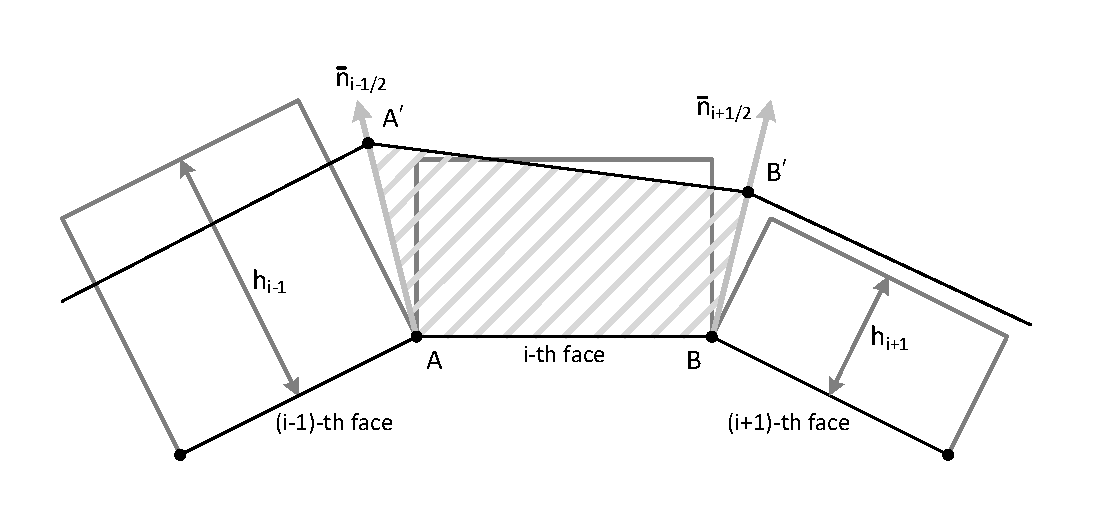
\includegraphics[width=0.8\textwidth]{pics/text_1_remesh_3d/pic_classical_methods_rectangles.pdf}
\caption{Перестроение поверхности с помощью метода прямоугольников в двумерном случае.}
\label{fig:text_1_remesh3_rect}
\end{figure}

\begin{figure}[ht]
\centering
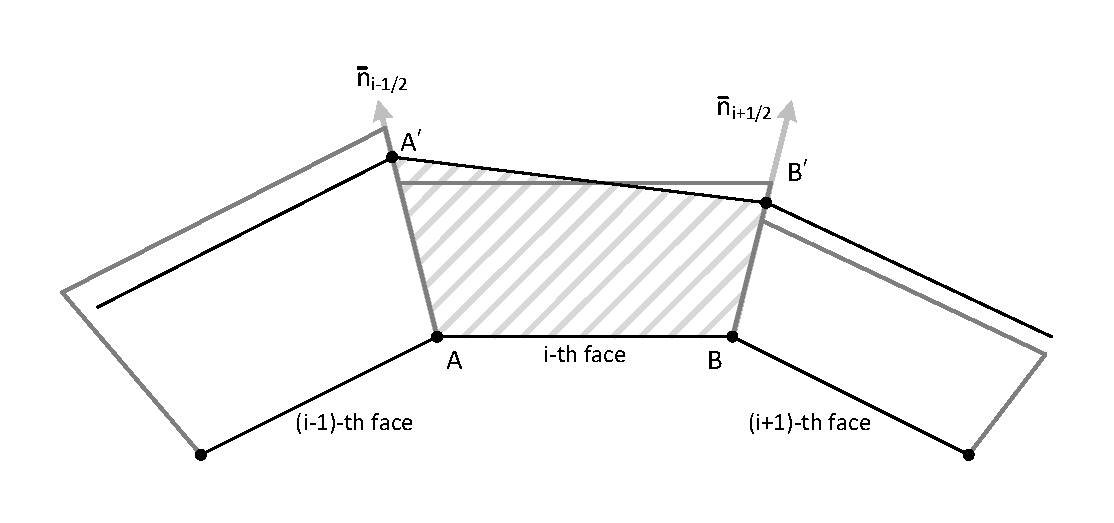
\includegraphics[width=0.8\textwidth]{pics/text_1_remesh_3d/pic_classical_methods_trapezoids.pdf}
\caption{Перестроение поверхности с помощью метода трапеций в двумерном случае.}
\label{fig:text_1_remesh3_trap}
\end{figure}

В качестве первого метода рассмотрим метод призм (в двумерной постановке аналогом данного метода является метод прямоугольников, продемонстрированный на рис.~\ref{fig:text_1_remesh3_rect}).
В этом методе входными данными является объем накопленного льда в каждой ячейке сетки ($V(f)$).
На первым шаге в каждой ячейке ищется толщина ледяного покрова в предположении, что лед в пределах одной ячейки имеет форму призмы, и ячейка является основанием этой призмы.
Тогда толщина ледяного покрова равняется $h(f) = \frac{V(f)}{S(f)}$, где $S(f)$ -- площадь ячейки.
После чего величина смещения каждого узла вычисляется просто как среднее арифметическое высот ледяного покрова во всех инцидентных ячейках:
\begin{equation}
h(N) = \frac{1}{|\mathscr{F}(N)|} \sum_{f \in \mathscr{F}(N)}{h(f)}.
\end{equation}

Второй метод можно назвать методом пирамид (в двумерной постановке аналогом данного метод является метод трапеций, показанный на рис.~\ref{fig:text_1_remesh3_trap}).
Входными данными также является объем накопленного льда в каждой ячейке сетки ($V(f)$).
Однако в отличие от предыдущего метода объем накопленного в ячейке льда представляется не призмой, а призматоидом, основанием которого является ячейка, а боковые ребра направлены вдоль нормалей узлов (мы будем условно называть эту фигуру усеченной пирамидой, чтобы не путать с методом призм, хотя в общем случае она усеченной пирамидой не является -- прямые, содержащие нормали трех инцидентных этой ячейке узлов, не обязаны пересекаться в одной точке).
Высота этой фигуры ищется из соотношений \eqref{eqn:text_1_geo_prim_abca1b1c1} с помощью решения кубического уравнения (решением является наименьший неотрицательный корень этого кубического уравнения).
Тогда как узлы ячейки являются точками первого основания построенной пирамиды, точки второго основания представляют собой новые положения узлов, вычисленные относительно рассматриваемой ячейки.
Таким образом, у каждого узла сетки вычисляется несколько новых положений (каждое из которых вычислено относительно своей инцидентной ячейки).
Для двумерного случая получается ровно два таких новых положения (так как в двумерном случае каждый узел имеет ровно две инцидентные ячейки), для трехмерного случае таких точек более двух.
Для выбора единственного нового положения узла сетки берется среднее значение из всех положений, вычисленных относительно инцидентных ячеек.

\begin{figure}[ht]
\centering
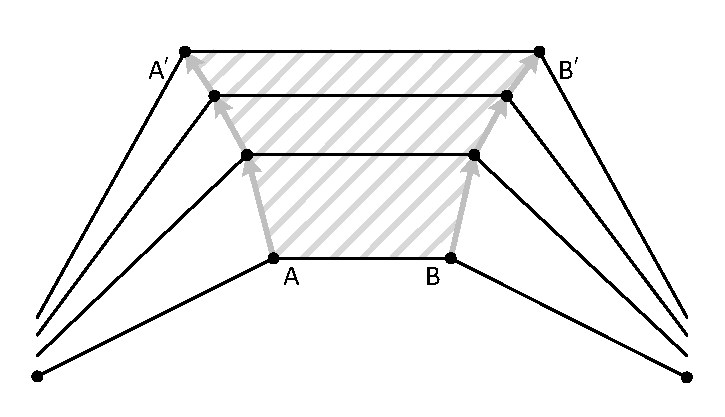
\includegraphics[width=0.6\textwidth]{pics/text_1_remesh_3d/pic_classical_methods_multilayer.pdf}
\captionstyle{center}\caption{Многослойное перестроение сетки.}
\label{fig:text_1_remesh3_multi}
\end{figure}

Вне зависимости от используемого метода перестроения значительно повысить точность перестроения можно с помощью многослойного подхода \cite{BourgaultCote2017}.
В этом случае вместо однократного перестроения сетки по объему накопленного льда в каждой ячейке ($V(f)$), выбирается фиксированное количество шагов перестроения $k$, а дальше процедура выполняется $k$ раз подряд, но с использованием объема накопленного в ячейке льда $\frac{V(f)}{k}$.
Точность повышается из-за того, что после каждого шага перестроения нормали в узлах сетки меняют свое направление, и общий объем наращиваемого льда становится более криволинейным, лучше учитывает геометрию сетки и, как следствие, точнее соответствует исходному значению $V(f)$ (см. рис.~\ref{fig:text_1_remesh3_multi}).

\subsubsection{Перестроение поверхности с сохранением объема}

В работах \cite{Thompson2013Remesh,Tong2017Remesh} описан устойчивый итерационный алгоритм эволюции поверхностной сетки, сохраняющий целевой объем льда.
В нем используется ряд улучшений по сравнению с классическими методами.

Многослойный подход, реализованный в этом методе, не использует константное количество шагов -- величина наращиваемого объема на каждом шаге алгоритма рассчитывается исходя из максимально допустимой доли временного шага обледенения, после превышения которого возможно развитие численной нестабильности в эволюции поверхности.
Наиболее очевидный случай возникает, когда проекции нормалей граней пересекаются, в этом случае слишком большой временной шаг приведет к складыванию поверхности.
Чтобы идентифицировать грани, которые будут демонстрировать подобное поведение на текущем временном шаге, предполагается, что объем, образованный путем вытягивания треугольной грани с использованием параллельной плоскости смещения, образует призматоид, объем которого определяется кубической функцией высоты $h$
\begin{equation}\label{text_1_remesh_3d_tong1}
V(h)=ah+bh^2+ch^3.
\end{equation}

где константы $a$, $b$, $c$ определяются позициями узлов грани, их нормалей и нормалью грани (вычисление этих коэффициентов приведено в \eqref{eqn:text_1_geo_prim_abca1b1c1}.

Рассмотрим корни квадратного уравнения, которое получается в результате дифференцирования уравнения \eqref{text_1_remesh_3d_tong1}.
Если корни являются положительными вещественными значениями, наименьший положительный корень определяет высоту, на которой достигается максимальный объем, которая обозначается как $V_{max}$, иначе функция $V(h)$ монотонно возрастает и ограничение на шаг в данной грани не требуется.
Исходя из этого, можно вычислить максимальную долю временного шага обледенения, которая требуется для обеспечения разумного поведения накопления объема.
В дополнение к этому пределу размера шага был введен предел стабильности $\alpha_{jiao}$, который основан на том, как изменяются направления нормалей по мере эволюции поверхности \cite{Jiao2007Offsetting}.
Тогда, допустимая доля временного шага для $i$-й грани определяется как
\begin{equation}
\alpha_{\Delta t}^i=
	\begin{cases}
		\min \left( s_{\Delta t} \frac{V_{\max}^i}{V_f}, \alpha_{jiao}, 1 \right), \ V_{\max}^i \ne \infty, \\
		\alpha_{jiao}, \ V_{\max}^i = \infty
	\end{cases}
\end{equation}

\

где $s_{\Delta t}$ ($0 < s_{\Delta t} < 1$) -- эмпирически определяемый коэффициент, $V_f$ -- текущий оставшийся объем приращения льда для $i$-й грани.
Тогда объем, наращенный для текущего шага, равен $\alpha_{\Delta t} V_f$, где $\alpha_{\Delta t}$ представляет собой глобальное минимальное значение для всех граней.

Другой важной особенностью алгоритма является введение первичного и нулевого простанств, описанных в \cite{Jiao2006Smooth}.
Если эволюционное движение узлов сетки происходит в первичном пространстве, то их перемещение в нулевом пространстве будет сохранять заметаемый объем, благодаря чему мы можем  проводить сглаживание поверхности сетки с сохранением объема.

В алгоритме используется несколько видов сглаживаний.
Первое сглаживание -- сглаживание нормалей в вершинах и ячейках сетки.
Чтобы сделать возможным сглаживание в нулевом пространстве, все нормали в узлах рассчитываются так, чтобы они лежали в первичном пространстве, а перемещение узлов при наращивании льда происходит только по их нормалям.
По мере эволюции, на поверхности может усиливаться шум -- если его не контролировать, может возникнуть ситуация, когда двугранный угол между гранями станет слишком малым и ограничит максимальную долю временного шага обледенения.
Для уменьшения поверхностного шума, перед наращиванием льда применяется локальное сглаживание, регулирующее направление смещения узла в проблемных областях, чтобы оно более точно совпадало с направлениями его соседей.
Этот метод может улучшить гладкость поверхности в некоторых ситуациях.
Основная цель сглаживания нормалей -- вытолкнуть точки из вогнутых областей, где нормали могут локально сходиться.
Сглаживание нормалей достигается с помощью серий взвешенных средних, которые предназначены для придания веса нормалям, генерируемым проблемными областями.

Второе сглаживание -- сглаживание высот.
После вычисления доли временного шага и объема, наращиваемого для текущего шага, для эволюции поверхности необходимо определить поле высот, которое будет соответствовать этому объему, чтобы по нему определить смещения узлов сетки.
Решение уравнения $V(h_i) = \alpha_{\Delta t} V_f$ обеспечивает поле начальных высот, которое используется для движения поверхности.
Цель дополнительного шага сглаживания высоты состоит в том, чтобы отфильтровать высокочастотный шум в поле высот за счет уменьшения разницы высот между соседними гранями.
Как правило, высоты двух треугольных граней, имеющих общее ребро, не будут равными.
На данном шаге используется сглаживание высот с сохранением объема путем его перераспределения между соседними гранями.

\begin{figure}[h]
\centering
\begin{tabular}{ll}
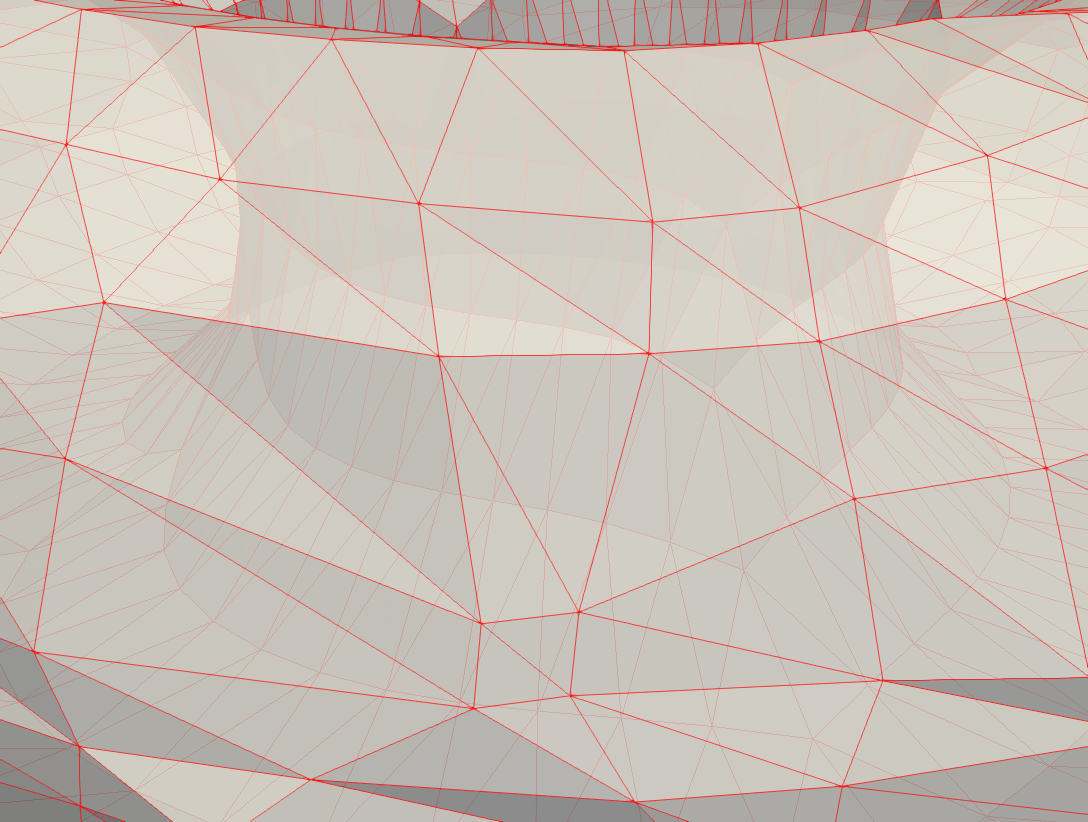
\includegraphics[width=0.45\textwidth]{pics/text_1_remesh_3d/pic_smooth_before.png}
&
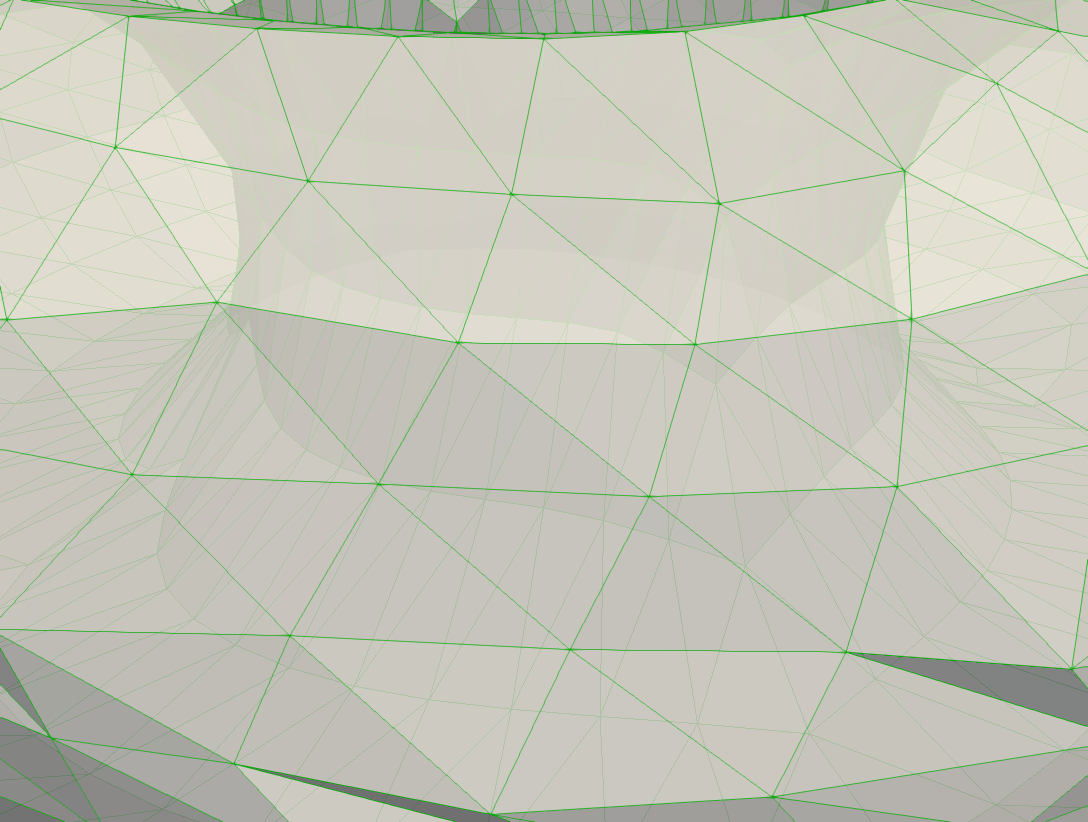
\includegraphics[width=0.45\textwidth]{pics/text_1_remesh_3d/pic_smooth_after.png}
\end{tabular}
\caption{Сглаживание в нулевом пространстве. Вид сетки до сглаживания (слева) и после (справа).}
\label{fig:text_1_remesh3_tong_smooth}
\end{figure}

Последним типом сглаживания является сглаживание в нулевом пространстве.
Эволюция поверхности будет стремиться упаковать узлы в вогнутые области, где сходятся нормали к поверхности, тогда как расширение сетки происходит в выпуклых областях, где нормали к поверхности расходятся.
Если узлы не будут перераспределены, может стать невозможным продолжать продуктивный, стабильный временной шаг.
Для улучшения качества поверхностной сетки узлы перераспределяются на поверхности с помощью сглаживания в нулевом пространстве.
Этот метод способен перераспределять точки, сохраняя при этом целостность базовой геометрии.
Нулевое пространство определяется касательной плоскостью (для гладких областей), касательной линией (для складок поверхности) или пустым пространством (для углов), движущиеся в нем узлы остаются на поверхности, так что объем и форма поверхности могут быть сохранены (\ref{fig:text_1_remesh3_tong_smooth}).
